\documentclass{article}
\usepackage[backend=bibtex]{biblatex}
\usepackage[UTF8]{ctex}
\usepackage{graphicx}
\usepackage{subfigure}
\usepackage{float}
\usepackage{amsfonts,amssymb}
\usepackage{ulem}
\title{论文笔记《Learning from Noisy Labels for Entity-centric Information Extraction》EMNLP2021}
\author{小十一}
\date{2021.11.13}
\usepackage[a4paper,left=10mm,right=10mm,top=15mm,bottom=15mm]{geometry} 

\begin{document}
\maketitle

\section{背景简介}
% \subsection{作者简介}
% \subsection{}
\begin{itemize}
   
    \item 大量的数据集中都有一定比例的噪声标签,影响了模型的性能。噪声对模型的影响主要来自两个方面:
          \begin{itemize}
              \item 噪声标签的分布和正确的标签分布不同,会影响模型推导   (incorrectly labeled instances are more likely to contradict the inductive bias captured by the model.) 对于噪声标签,模型要花更多的时间把它找出来。
              \item 在模型的训练过程中,模型会很快遗忘这个噪声标签带来的信息或者说忘记见过这个错误打标的实例。
          \end{itemize}
\end{itemize}
作者提出提出问题:如何构建一个 noise-robust IE 模型?现有方法主要是关注弱监督或者远监督(多实例学习)。作者指出这种外部资源并不总是现成,不能很好地迁移到现存的有监督模型训练上。
作者提出的方法是用 一个 task-specific loss 训练模型和一个 agreement loss 去约束模型。
\begin{itemize}
    \item \textbf{task-specific loss}: 训练模型去拟合标签。但是单纯使用这个 loss 的话,模型会把噪声也一视同仁的拟合,影响模型效率。
    \item \textbf{agreement loss}: 出发点是对于噪声标签,多个模型可能会给出不一致的预测。于是作者把这种多个模型预测不一致的实例当作噪声,对于噪声实例,agreement loss 鼓励多个模型之间达到一致,而不是去和错误的 ground truth label 保持一致(\textbf{论文的创新})。
\end{itemize}


\section{相关工作}
两个方面: 
\begin{itemize}
    \item distant supervision
    \item supervised learning with noisy labels (most relative). 主要说了一些图像上的工作: robust loss function, noisy filter layer, label-reweighting, robust regularization, sample selection. 
    \begin{itemize}
        \item 前两个都需要修改模型结构,不适合直接迁移到 IE 模型上。 \item Sample selection 方法认为带有最大 training loss 的实例是噪声,并把它从训练数据中去掉。但是长尾分布的实例由于样本较少,也很可能出现较大的 train loss ,会被模型错误地排除,从而导致性能下降。
        \item CrossWeigh 通过给实例不同的训练权重来降低噪声对模型带来的影响,但是计算量大。详细做法:把训练集分成10个块,把其中的9个用来做训练集独立训练三个模型,然后这三个模型对剩下的块中实例进行预测。如果模型预测不一致,就降低这个实例的权重。这样一来,为了给所有训练集中实例一个权重,需要训练30个独立的模型,计算量大。
    \end{itemize}
\end{itemize}

\section{方法}
\subsection{依据}
在有噪声的数据上,学习曲线会先增加后下降。原因是:
\begin{itemize}
    \item On noisy data, neural models tend to fit easy and clean instances that are more consistent with the well-represented patterns of data in early steps but need more steps to capture noise.
    \item The learned noisy examples tend to be frequently forgotten in later epochs since they conflict with the general inductive bias represented by the clean data majority.
\end{itemize}
因此,多个模型对于干净的数据预测基本一致,但是对于噪声数据的预测很有可能不一致或者振荡(振荡是说的模型的前后预测)。所以现有方法对于模型预测不一致的实例都降低权重或者更正标签以减少它们的影响。

\subsection{整体框架}
作者提出的方法总体框架图如\ref{framework}所示。
\begin{figure}[H]
    \centering
    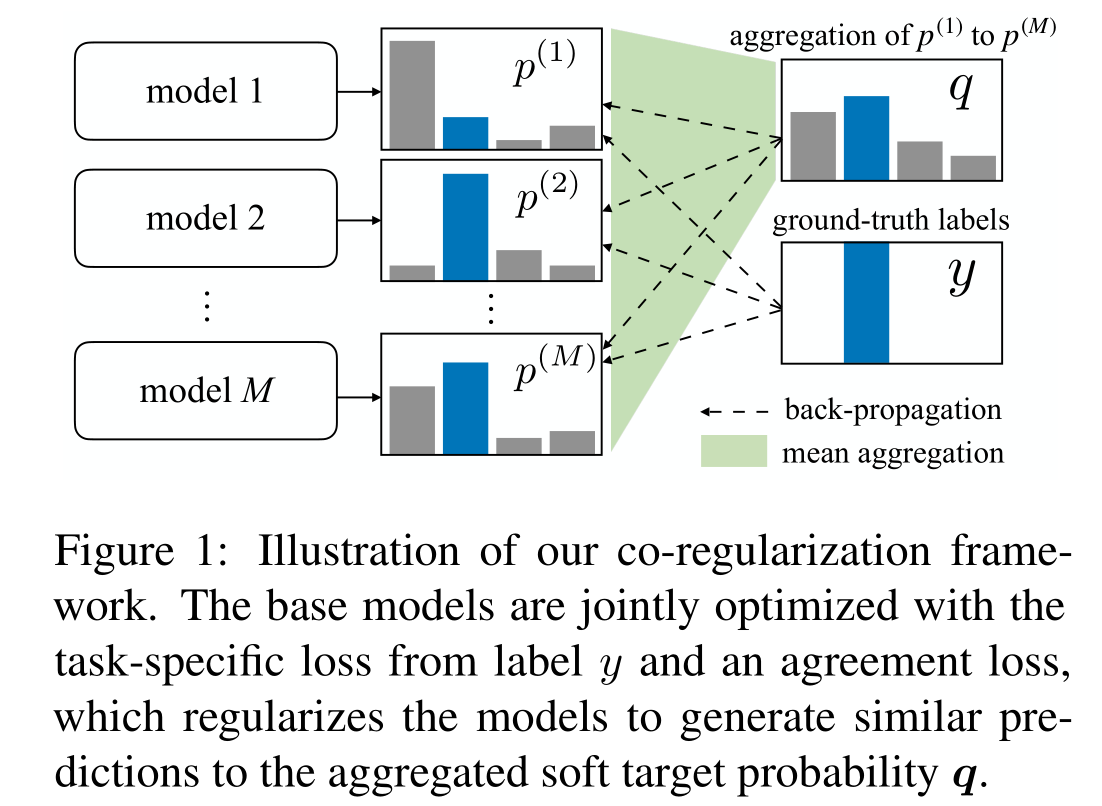
\includegraphics[width=0.8\textwidth]{fig/framework.png}
    \caption{框架图}
    \label{framework}
\end{figure}

随机初始化多个模型,然后分两阶段训练,首先只用 task-specific loss 对模型进行训练,要求模型拥有正确预测标签的能力,类似 warm up 阶段。然后在用 agreement loss 联合训练模型,要求模型在面对预测不一致的样本(噪声实例)时,保持和 soft target distribution 一致,而不是和错误的 ground truth 一致。具体算法如图\ref{algorithm}所示
\begin{figure}[H]
    \centering
    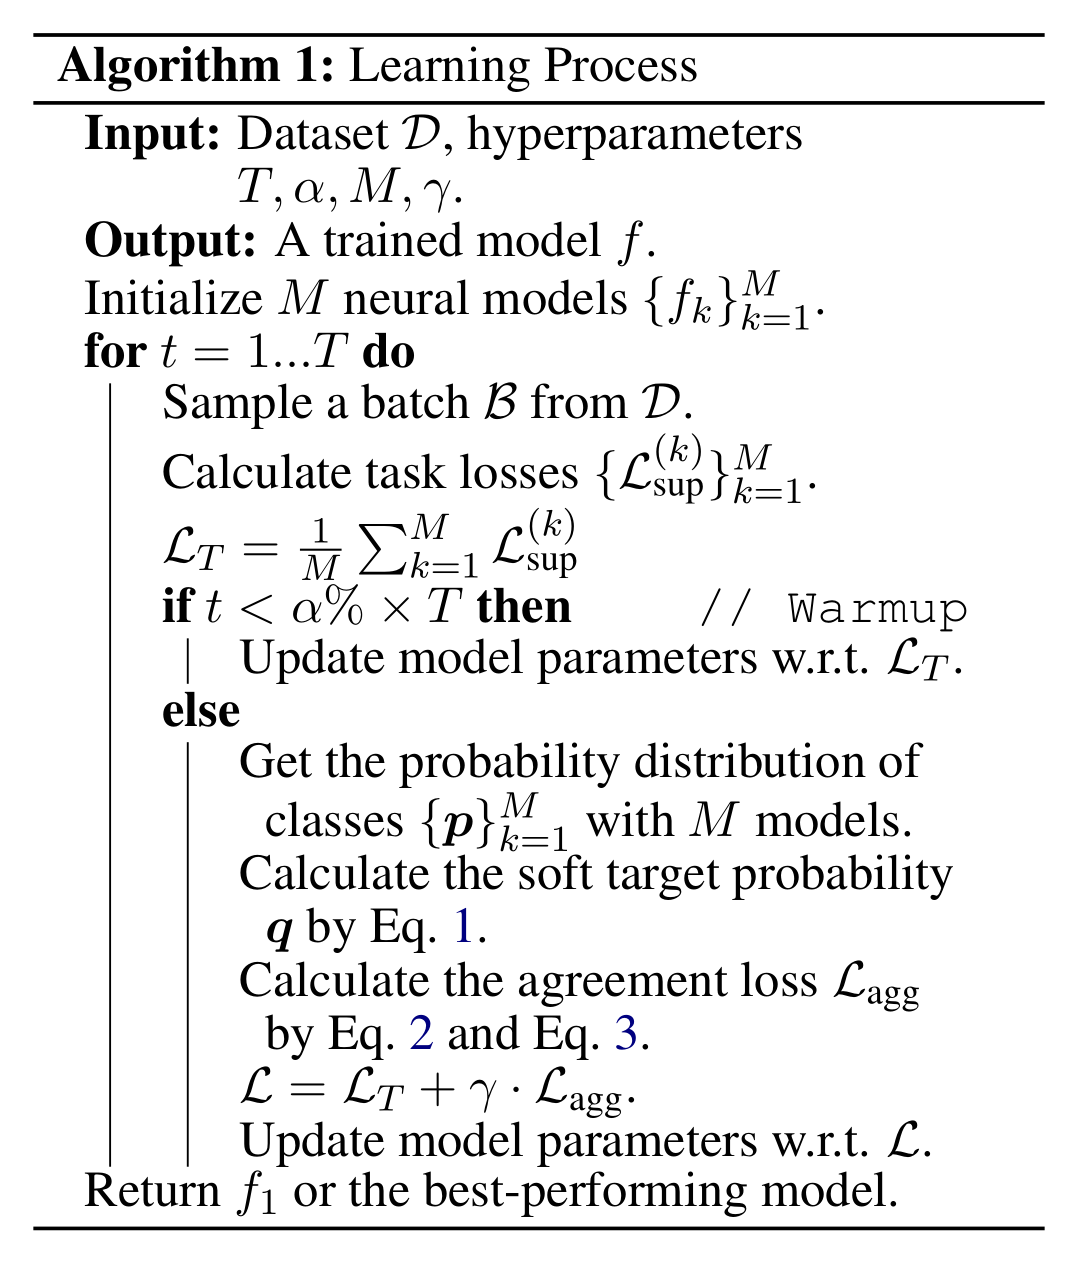
\includegraphics[width=0.8\textwidth]{fig/algorithm.png}
    \caption{整体算法}
    \label{algorithm}
\end{figure}

其中的$q$表示soft target distribution ,计算过程如公式(\ref{eq1}):
\begin{equation}
    q_i=\frac{1}{M}\sum_{k=1}^{M}{p_i^{(k)}} \label{eq1}
\end{equation}
其中的$M$表示模型的数量,$p_i^{(k)}\in \mathbb{R}^C$表示第$k$个模型对第$i$个样本的预测。$C$是分类类别数目。


PS: 当时读论文的时候还在想,居然只用简单的平均,虽然平均确实可以消除误差,但应该还有更好的方法吧,比如如果模型经常振荡,给一下比较小的权重之类的,或者动态权重什么的。当时还以为作者没有考虑那么多,其实不然,自己还是非常的浅薄呀。这里用平均其实是考虑了后面 KL 散度的计算。继续往下看吧。

最重要的 agreement loss 的设计其实并不复杂,就是一个度量两个分布之间距离的 KL 散度。 $\mathcal{L}_{agg}$的计算如公式(\ref{eq2})、(\ref{eq3})所示。
\begin{equation}
    d(q_i||p_i^{(k)}) = \sum_{j=1}^{C}{q_{ij}log(\frac{q_{ij}+\epsilon}{p_{ij}+\epsilon})}
    \label{eq2}
\end{equation}
\begin{equation}
    \mathcal{L}_{agg} = \frac{1}{MN} \sum_{k=1}^{M}{\sum_{i=1}^{N}{d(q_i||p_i^{(k)})}}
    \label{eq3}
\end{equation}
其中的$\epsilon$是为了防止除0。

个人感觉公式(3)写成这样更好理解一点,计算每个模型的分布和 soft target distribution 之间的距离,然后求和。原文中的公式(3)如下:
\begin{equation}
    \mathcal{L}_{agg} = \frac{1}{MN} \sum_{i=1}^{N}{\sum_{k=1}^{M}{d(q_i||p_i^{(k)})}}
    % \label{eq3}
\end{equation}

虽然计算简单,但是很巧妙,很容易可以看出$\mathcal{L}_{agg}$鼓励模型对于相同的输入应该有相似的输出。由于 KL 散度是非负的,只有当$q_i=p_i^{(k)}, k=1,2,\ldots,M$时,$\mathcal{L}_{agg}$最小。这就表示了$p_i^{(k)}$应该一致且等于$q_i$,所以之前$q$的表示用了平均值。作者提到其实只要满足:当所有的$p_i^{(k)}$相等时,有$q_i=p_i^{(k)}, k=1,2,\ldots,M$成立,就可以了。所以又提出了两种得到$q$的方法:
\begin{itemize}
    \item Average logits: 就是对模型没有经过 softmax 之间的输出值进行平均
    \item Max-loss probability: 一个好的 noise-robust model 会和 noise label 非常不一致,从而产生较大的 task-specific loss. 所以对于每一个批次中的每一个实例,带有最大 task-specific loss 的预测最可靠,然后用这个实例的预测当成这个实例的 soft target distribution.(但是 task-specific loss 大的话也不能表明一定是噪声吧,可能就是那个实例复杂导致模型不能正确分类)
\end{itemize}
后面证实:这几种策略效果差异不大。

\subsection{联合训练}
主要的就是优化 $\mathcal{L}=\mathcal{L}_T+\gamma \mathcal{L}_{agg}$,其中$\gamma$是超参数,$\mathcal{L}_T$是 task-specific loss.
task-specific loss 计算如下:
\begin{equation}
    \mathcal{L}_{T} = -\frac{1}{M}\sum_{k=1}^{M}{ \mathcal{L}_{sup}^{(k)} }
    \label{eq5}
\end{equation}

\begin{equation}
    \mathcal{L}_{sup}^{(k)} = -\frac{1}{N}\sum_{i=1}^{N}{\sum_{j=1}^{C}{I[y_i=j]log{p_{ij}^{(k)}}}}
    \label{eq6}
\end{equation}

其中$I$表示指示函数。

这样联合训练的好处在于,对于干净的标签,模型预测都比较一致,$\mathcal{L}_{agg}$值非常小,不会对模型优化产生影响;但是对于噪声标签,模型之间会变得不一致,$\mathcal{L}_{agg}$会变大,防止模型过度拟合噪声标签。这样比直接剪枝掉 task-specific loss 大的实例更好,因为这样的剪枝策略会把服从长尾分布的实例剪掉。(作者做实验发现的)



\section{实验}

实验主要包含两个任务:NER和RE,数据集分别是噪声数据集CoNLL03和TACRED。
NER的实验结果如图\ref{table1}所示。RE的实验结果如图\ref{table2}所示。
\begin{figure}[H]
    \centering
    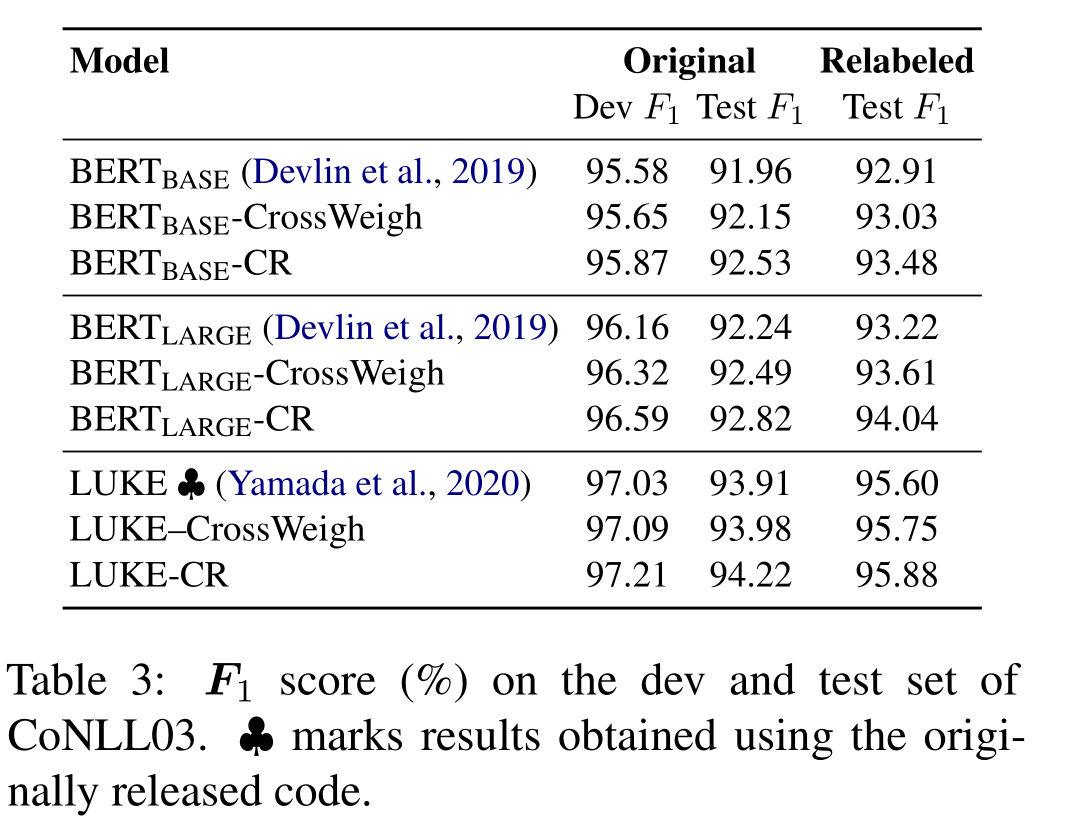
\includegraphics[width=.8\textwidth]{fig/main result ner.png}
    \caption{NER实验结果}
    \label{table1}
\end{figure}

\begin{figure}[H]
    \centering
    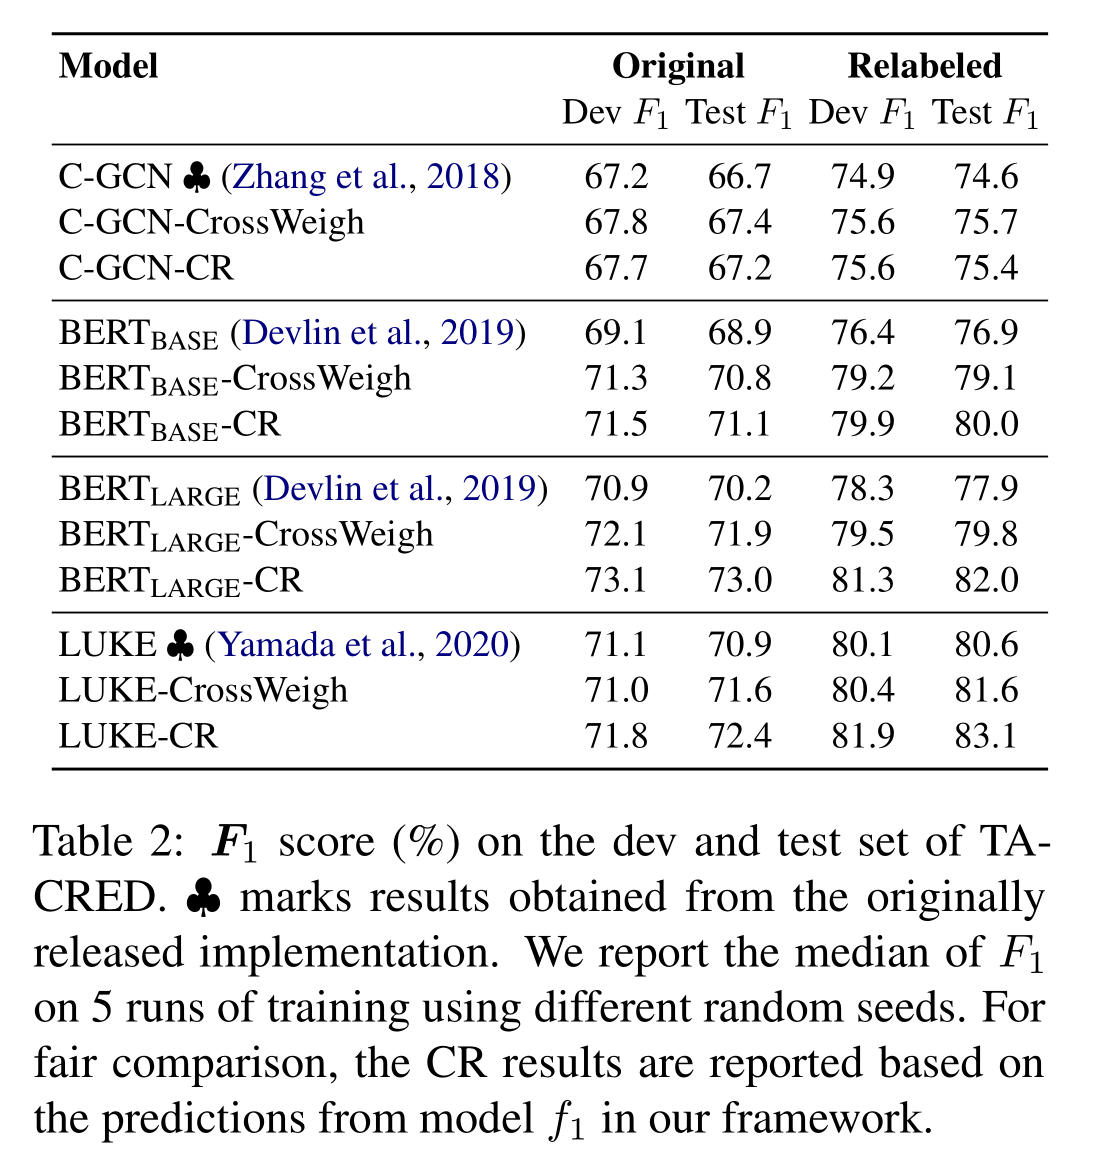
\includegraphics[width=.8\textwidth]{fig/main result1.png}
    \caption{RE实验结果}
    \label{table2}
\end{figure}

实验结果总结:
\begin{enumerate}
    \item 模型确实有一些提升。
    \item 噪声过滤的实验证明$\mathcal{L}_{agg}$的有效性,尤其对于拟合能力比较强的模型。\textbf{有趣的是,按照这样的说法,bert拟合能力太强,对噪声也拟合了。但是图\ref{table2}中BERT的效果还是比GCN好。有点一个好的降噪方法还是不如一个拟合能力更强的模型的意思了。}
    \item 使用其他噪音数据的剪枝策略(hard prune)没有给模型带来明显提升,作者实验发现是简直了长尾分布的数据。而作者提出的方法防止了这一错误,比它们大概有两个点提升。
    \item 增加模型数量没有明显提升,甚至在bert-base上下降了。
    \item 增加数据集中的噪声比例,随着噪声变多,作者提出的方法性能下降比CrossWeigh会更慢。
\end{enumerate}

\begin{itemize}
    \item 方法中 warm up 阶段说到了调节$\alpha$,但是实验中没有给出关于它的参数敏感实验。也没说最后把$\alpha$设置成了多少。
    \item 
\end{itemize}

\section{思考}

\begin{itemize}
    \item 只有做实验才能知道别人的缺点在哪里,多思考,不要想当然。把别人的模型拿到其他数据集(比如说有其他特点,噪声很大,或者长尾分布很严重,或者样本少)上跑一跑,看看能不能 work ,分析为什么能又为什么不能,把 learning curve, loss 什么的都打印出来看看?例如作者发现 hard prune 会影响到长尾分布数据。
    \item 作者在推断的时候选择的是在dev上表现得最好的模型,而按照学习曲线来说,这个模型应该会在训练的较早阶段得到,而文中2.1节中说到模型在训练前期很容易拟合到简单且干净的标签,这个时候得到的模型真的能够排除训练集中噪声的影响吗?还是说噪声都还没来得及影响模型,模型就保存,然后拿去推断了。
\end{itemize}
\end{document}